\section{直言命题的符号系统与图解}

\begin{quotation}
布尔解释为直言命题提供了严谨的基础,但为了更直观地理解命题间的关系,我们需要一套符号系统和图解方法。本节介绍如何用代数符号表示直言命题,以及如何用文恩图直观展示命题的含义和相互关系,为下一章分析三段论有效性奠定基础。
\end{quotation}

直言命题的布尔解释在很大程度上以\textbf{空类}概念为基础,为方便起见,可用一个特殊的符号来表示空类。此处我们用数字"0"来代表空类。说词项$S$指称的类没有元素,就在$S$和0之间划上等号。也就是说,$S=0$表示$S$没有元素($S$的元素$s$简记为$S^{\prime}s$,说不存在$S^{\prime}s$亦即$S=0$)。

说$S$指称的类确实有元素就是否定$S$为空。断定"存在$S$′$s$"就是对$S=0$所表示的命题的否定。我们在等号上加一条斜线表示这种否定式。就是说,$S \neq 0$表示存在$S$′$s$,是对$S$为空的否定。

\subsection{直言命题的符号表示}

标准式命题都涉及两个类,所以表示它们的等式要复杂一些。两个类都分别由一个符号代表,因此可以把两个符号并排在一起,用以表示那些由同时属于两个类的元素组成的类。比如,如果$S$代表所有"讽刺作品"组成的类,$P$代表所有"诗"组成的类,那么,既是讽刺作品又是诗的东西组成的类就可以用符号$SP$表示,它代表的就是所有讽刺诗(或者说诗式讽刺作品)组成的类。两个类的共同部分或全体共同元素称为两个类的\textbf{积}(product)或\textbf{交}(intersection)。两个类的积是所有同时属于这两个类的东西组成的类。所有美国人的类与所有作家的类之积就是所有美国作家的类。(此处必须与自然语言的某些特定用法区分开来。例如,西班牙人的类与舞蹈家的类之积,不是西班牙舞蹈家的类,因为通常说的西班牙舞蹈家不是西班牙的舞蹈家,而是表演西班牙舞蹈的人。同样,抽象画家、英语课程、古董商人等等也都是这样的用法。)

使用这种新记法,我们也可以用等式和不等式将E和I命题符号化。E命题"没有$S$是$P$"说的是$S$类中没有元素是$P$类的元素,即没有东西同时属于两者。换言之,两个类的积为空,可用等式符号表示为:$SP=0$。I命题"有$S$是$P$"说的是$S$类中至少有一个元素也是$P$类的元素。这意味着$S$类和$P$类的积不空,可用不等式符号表示为:$SP \neq 0$。

对于A命题和O命题,需要引人一个表示\textbf{补类}的新方法。如5.5节所说明,一个类的补类就是所有那些不属于原类的东西的类或汇集。例如,士兵的类的补类就是所有不是士兵的东西组成的类,即非士兵的类。若用$S$代表士兵的类,则把非士兵的类记为:$\bar{S}$(读做:$S$杠),即在原来的类之上加一横杠。A命题"所有$S$是$P$"说的是$S$类的所有元素都是$P$类的元素,也就是说,没有$S$类的元素不是$P$类的元素。或者说(据换质法)"没有$S$是非$P$",像任何E命题一样,这个命题说的是,主项指称的类与谓项指称的类的积为空,可用等式符号表示为:$S\bar{P}=0$。O命题"有$S$不是$P$"换质后得逻辑等价式I命题"有$S$是非$P$",可用等式符号表示为:$S\bar{P} \neq 0$。

使用这些符号公式,就能很清晰地显示四种标准式直言命题之间的相互关系。既然A命题和O命题的符号公式分别为$S\bar{P}=0$和$S\bar{P} \neq 0$,它们显然是互为矛盾的。E命题和I命题的符号形式分别为:$SP=0$和$SP \neq 0$,显然也是互为矛盾的。布尔解释下的对当方阵可以重新表示为图5-2。

\subsection{文恩图及其应用}

命题可以用所涉及的类的图示来表达。我们用一个圆代表一个类,用指称类的词项标注它。这样$S$类可以表示为图5-3。

\begin{center}
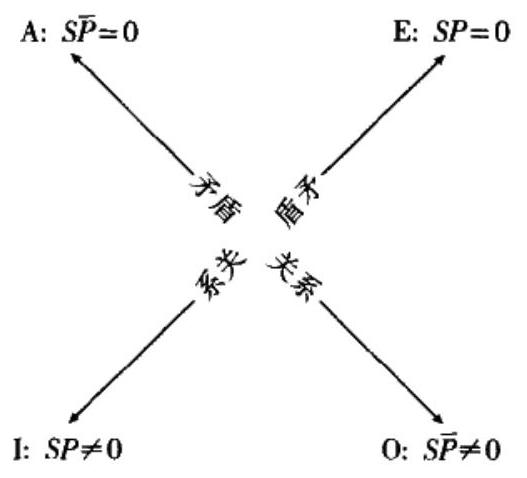
\includegraphics[width=\textwidth]{images/2025_05_15_6a28331d5e7c993ad07ag-257(2).jpg}

图5-2 布尔解释下的对当方阵
\end{center}

\begin{center}
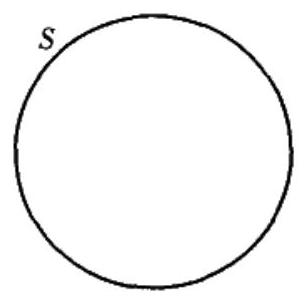
\includegraphics[width=\textwidth]{images/2025_05_15_6a28331d5e7c993ad07ag-257.jpg}

图5-3 类的图示
\end{center}

上图表示的是一个类,而不是命题。它只代表$S$类,而对这个类无所言说。要图示命题"$S$没有元素"或"不存在$S$′$s$",我们就在代表$S$的圆中加上阴影,来表示$S$中什么都没有,$S$为空类。要图示"存在$S$′$s$"这个命题,我们就在代表$S$的圆中写一个$x$,用来表示其中有东西,$S$不是空类。这样,"不存在$S$′$s$"和"存在$S$′$s$"这两个命题就可以用图5-4来表示。

\begin{center}
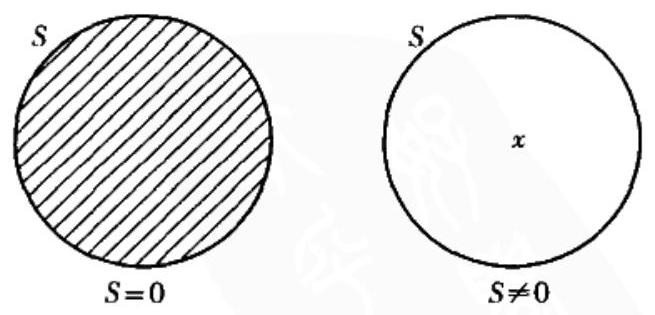
\includegraphics[width=\textwidth]{images/2025_05_15_6a28331d5e7c993ad07ag-257(1).jpg}

图5-4 空类与非空类的图示
\end{center}

实际上,表示$S$的图示也可以表示$\bar{S}$,因为圆中的部分代表的是$S$的所有元素,而圆外的部分恰好就是$\bar{S}$。

要图示标准式直言命题,一个圆不够,而需要两个圆。标准式直言命题的主、谓项分别记为$S$和$P$,而后画两个相交的圆,如图5-5。

\begin{center}
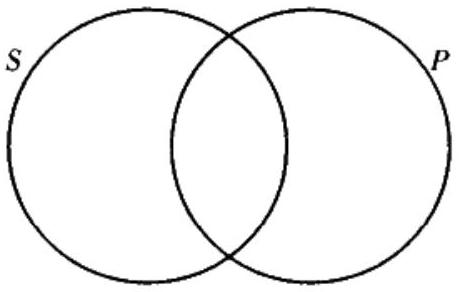
\includegraphics[width=\textwidth]{images/2025_05_15_6a28331d5e7c993ad07ag-258.jpg}

图5-5 两个类的图示
\end{center}

图示只表示出了$S$和$P$两个类,而没有表示它们形成的命题。既没有肯定也没有否定其中一个或两个类有元素。实际上,两个相交的圆表示出的类不只是$S$和$P$两个。标有$S$的圆中与$P$不重叠的部分代表的是所有不是$P$′$s$的$S$′$s$,即代表了$S$类与$\bar{P}$类的积,这一部分标记为$S\bar{P}$。两圆相交的部分代表$S$类与$P$类的积,标记为$SP$。标有$P$的圆中与$S$不重叠的部分代表的是所有不是$S$′$s$的$P$′$s$,即代表了$\bar{S}$类与$P$类的积,标记为$\bar{S}P$。最后,两个圆之外的部分,代表既不在$S$类也不在$P$类之中的东西,标记为第四个类$\overline{SP}$。加上这些标记,图5-5就成了图5-6:

\begin{center}
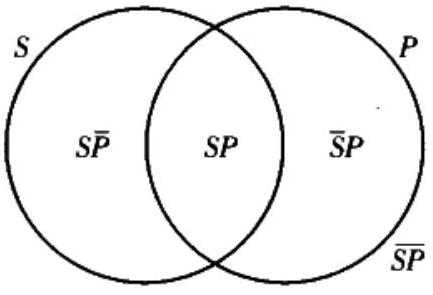
\includegraphics[width=\textwidth]{images/2025_05_15_6a28331d5e7c993ad07ag-258(1).jpg}

图5-6 文恩图中的四个类区域
\end{center}

可以用各种不同的类来解释上图。例如设西班牙人的类为$S$、画家的类为$P$,则$SP$就是两个类的积,由所有同时属于两个类的东西组成。因为$SP$的每个元素必须既是$S$类也是$P$类的元素,所以每个元素既是西班牙人又是画家。两个类的积就是西班牙画家的类,其中包括委拉斯开兹(Velásquez)和戈雅(Goya)等人。$S\bar{P}$是第一个类与第二个类之补的积,包括且只包括属于$S$类但不属于$P$类的对象,也就是不是画家的西班牙人组成的类,即所有非画家西班牙人,委拉斯开兹不在其中,戈雅也不在其中,但却包括小说家塞万提斯(Cervantes)和独裁者佛朗哥(Franco)及其他西班牙人。$\bar{S}P$是第二个类与第一个类之补的积,是那些不是西班牙人的画家组成的类,这个类包括荷兰画家伦布兰特(Rembrandt)、美国画家乔治亚•奥基夫(Georgia O'Keeffe)等。最后,$\overline{SP}$是原来两个类的补的积,包括而且只包括那些既不是西班牙人也不是画家的对象。这可是一个很大的类,包括的不只是英国海军上将和瑞士登山运动员们,还包括诸如密西西比河、珠穆朗玛峰这样的东西。如果对$S$和$P$进行这样的解释,那么,以上说的所有类都在图5-6中有所表示。

这就是\textbf{文恩图}(Venn diagram),得名于英国数学家、逻辑学家约翰•文恩(John Venn,1834-1923),他首先使用这种方法表示类和命题。像图5-6这样的带有几处标记的双圆图,所代表的仍只是类,尚不表示任何命题。整个圆或其中留做空白的部分既不表示类中有元素,也不表示没有。

但是,再加上一定条件,我们就能用文恩图来表示命题。通过给某些部分加上阴影,或者标上"$x$",就能准确地将四种标准式直言命题图示化。文恩图(带有标记的)能够全面、简明地表示命题,所以,它已经被公认为评价三段论论证的最有力、使用最广泛的方法。下面就来说明如何用文恩图表示这四种标准式命题。

A命题"所有$S$是$P$"即$S\bar{P}=0$,用文恩图图示之,可把代表$S\bar{P}$的那部分加上阴影,即表示其中没有元素。E命题"没有$S$是$P$"即$SP=0$,可把图中代表$SP$的那部分加上阴影,以示其中没有元素。I命题"有$S$是$P$"即$SP \neq 0$,可在图中$SP$类部分标上一个$x$,表示两个类的积不是空的,其中至少有一个元素。最后,O命题"有$S$不是$P$"即$S\bar{P} \neq 0$,可加一个$x$在$S\bar{P}$部分,表示其中至少有一个元素而不是空的。将以上四个图示列在一起,就能十分清晰地展现出四种命题的不同含义,见下图5-7。

我们已经用文恩图表示出"没有$S$是$P$"和"有$S$是$P$",而它们换位后分别得到一个等价命题:"没有$P$是$S$"和"有$P$是$S$",因此后面两个命题在图中也就表示出来了。要图示A命题"所有$P$是$S$"即$P\bar{S}=0$,循同样路径,可把代表$P\bar{S}$的部分加上阴影。显然,$P\bar{S}$与$\bar{S}P$是相同的,如果一下子不能明白,就回想一下是画家而非西班牙人的类,与非西班牙人中是画家的类。前一个类中的对象必定也是后一个类的对象——即所有是画家而非西班牙人的人与所有非西班牙人的画家,反之亦然。要图示命题"有$P$不是$S$"即$P\bar{S} \neq 0$,可在$P\bar{S}(=\bar{S}P)$部分加上一个$x$。图5-8展示的正是这几个命题。

\begin{center}
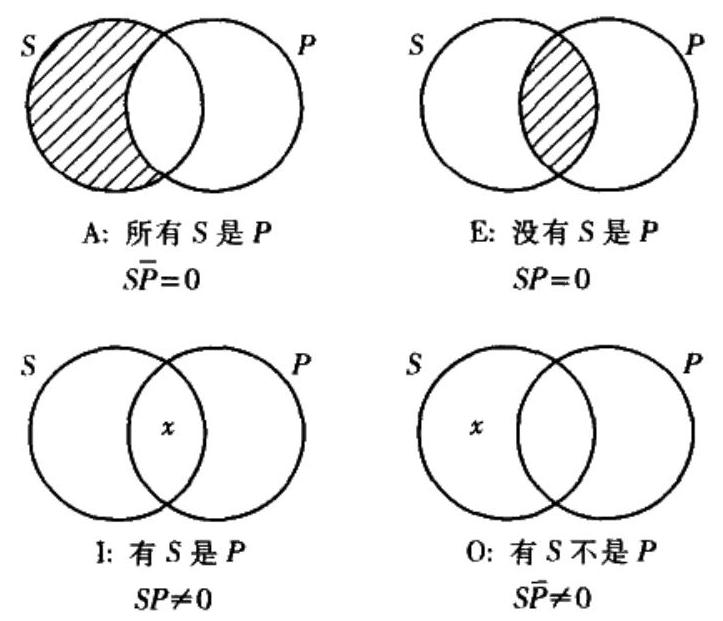
\includegraphics[width=\textwidth]{images/2025_05_15_6a28331d5e7c993ad07ag-260(1).jpg}

图5-7 四种标准式命题的文恩图
\end{center}

\begin{center}
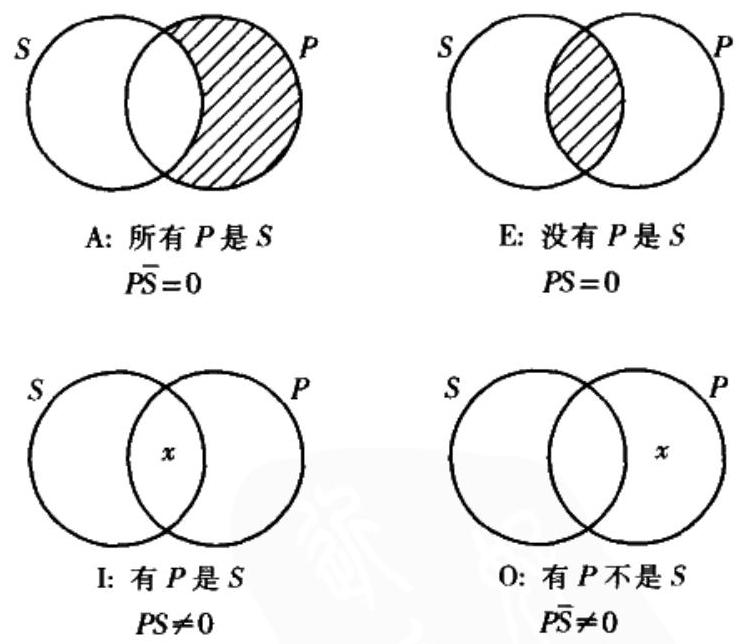
\includegraphics[width=\textwidth]{images/2025_05_15_6a28331d5e7c993ad07ag-260.jpg}

图5-8 更多命题的文恩图表示
\end{center}

双圆图的这种灵活运用,在本书下一章中起着重要作用。任给一对带有给定标记——比如$S$和$M$——的交叉圆,就能将任何一个含有$S$和$M$的标准式直言命题图示化,无论$S$和$M$出现的顺序如何。

文恩图是标准式直言命题的肖像,将空间的包含与排斥与类间非空间的包含与排斥对应起来,是一种极为清晰的记法。下一章将会看到,这也是检验直言三段论的有效性的一种最简单、最直接的方法。

\begin{center}
\fbox{\parbox{0.95\textwidth}{
\textbf{本节要点}
\begin{itemize}
\item \textbf{直言命题的符号表示}
  \begin{itemize}
  \item 空类用"0"表示,$S=0$表示类$S$没有元素
  \item 非空类用$S \neq 0$表示,表示类$S$至少有一个元素
  \item 类的积(或交)记为$SP$,表示同时属于$S$和$P$的元素组成的类
  \item 类的补记为$\bar{S}$,表示不属于类$S$的所有元素
  \item 四种标准式命题的符号表示:
    \begin{itemize}
    \item A命题:"所有$S$是$P$"$\Rightarrow$ $S\bar{P}=0$
    \item E命题:"没有$S$是$P$"$\Rightarrow$ $SP=0$
    \item I命题:"有$S$是$P$"$\Rightarrow$ $SP \neq 0$
    \item O命题:"有$S$不是$P$"$\Rightarrow$ $S\bar{P} \neq 0$
    \end{itemize}
  \end{itemize}
\item \textbf{文恩图}:用图形直观表示命题的方法
  \begin{itemize}
  \item 圆形代表类,重叠部分代表类的交
  \item 阴影表示该区域为空类
  \item 带"$x$"标记表示该区域非空
  \item 文恩图能直观展示命题间的关系,是检验三段论有效性的有力工具
  \end{itemize}
\end{itemize}
}}
\end{center} 